\subsubsection{Q10.14 data 10312021 11092021 grouped by scenario}

\begin{comment}
               EFPR        EO      EFNR     n    pvalue
(frauth,)  0.380952  0.619048  0.464286  42.0  0.092180
(icu,)     0.486111  0.513889  0.569444  36.0  0.533588
(rent,)    0.397436  0.602564  0.423077  39.0  0.186486
\end{comment}

\begin{table}[h]
    \centering
    \begin{tabular}{|c|c|c|c|c|c|}
        \hline
        scenario & EFPR & EO & EFNR & n & p-value\\
        \hline
        frauth & 0.381 & \textbf{0.619} & 0.464 & 42.0 & 0.092\\
		icu & 0.486 & \textbf{0.514} & \textbf{0.569} & 36.0 & 0.534\\
		rent & 0.397 & \textbf{0.603} & 0.423 & 39.0 & 0.186\\
		
        \hline
    \end{tabular}
    \caption{Grouped by scenario}
    \label{tab:my_label}
\end{table}
\begin{figure}[h]
    \centering
    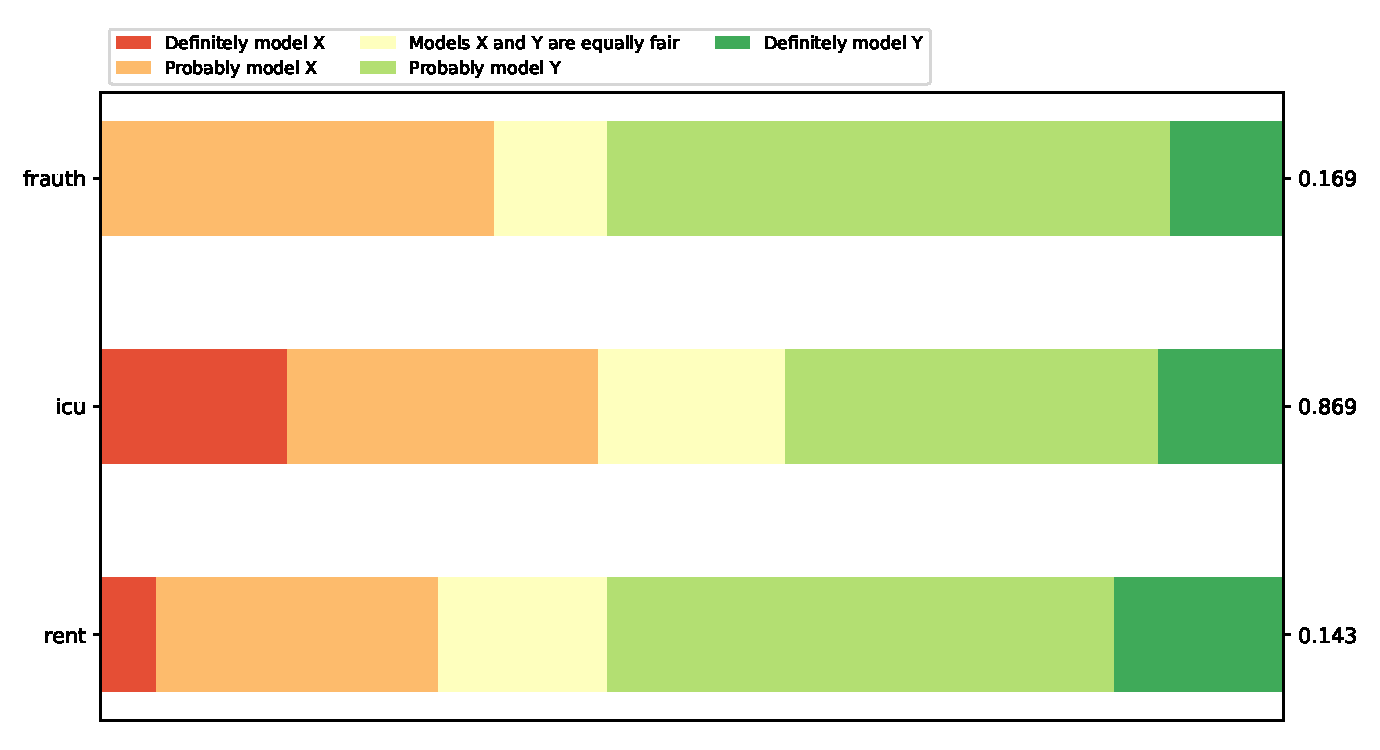
\includegraphics[width=0.8\textwidth]{figures/Q10.14/10312021_11092021/Q10.14_scenario.pdf}
    \caption{Grouped by scenario}
    \label{fig:my_label}
\end{figure}
